\subsection{Aufbau und Durchführung des Versuchs V501}
\subsubsection{Proportionalität der Ablenkung und der Ablenkungsspannung}
In einer Kathodenstrahlröhre gibt es zunächst eine Glühwendel, aus der die negativ geladenen Elektronen emittiert werden.
Die Elektronen werden anschließend durch eine negativ geladene Blende, den Wehnelt-Zylinder, grob fokussiert und dann durch eine stark positiv geladene Elektrode beschleunigt.
Die genauere Fokussierung erfolgt durch mehrere negativ geladene Fokussierungselektroden (Abb. \ref{fig:KSR}).
Die Elektronen durchlaufen danach die beiden Ablenkungskondensatoren.
Die Ablenkung findet in X-Richtung und analog in Y-Richtung statt.
\begin{figure}[h!]
  \centering
  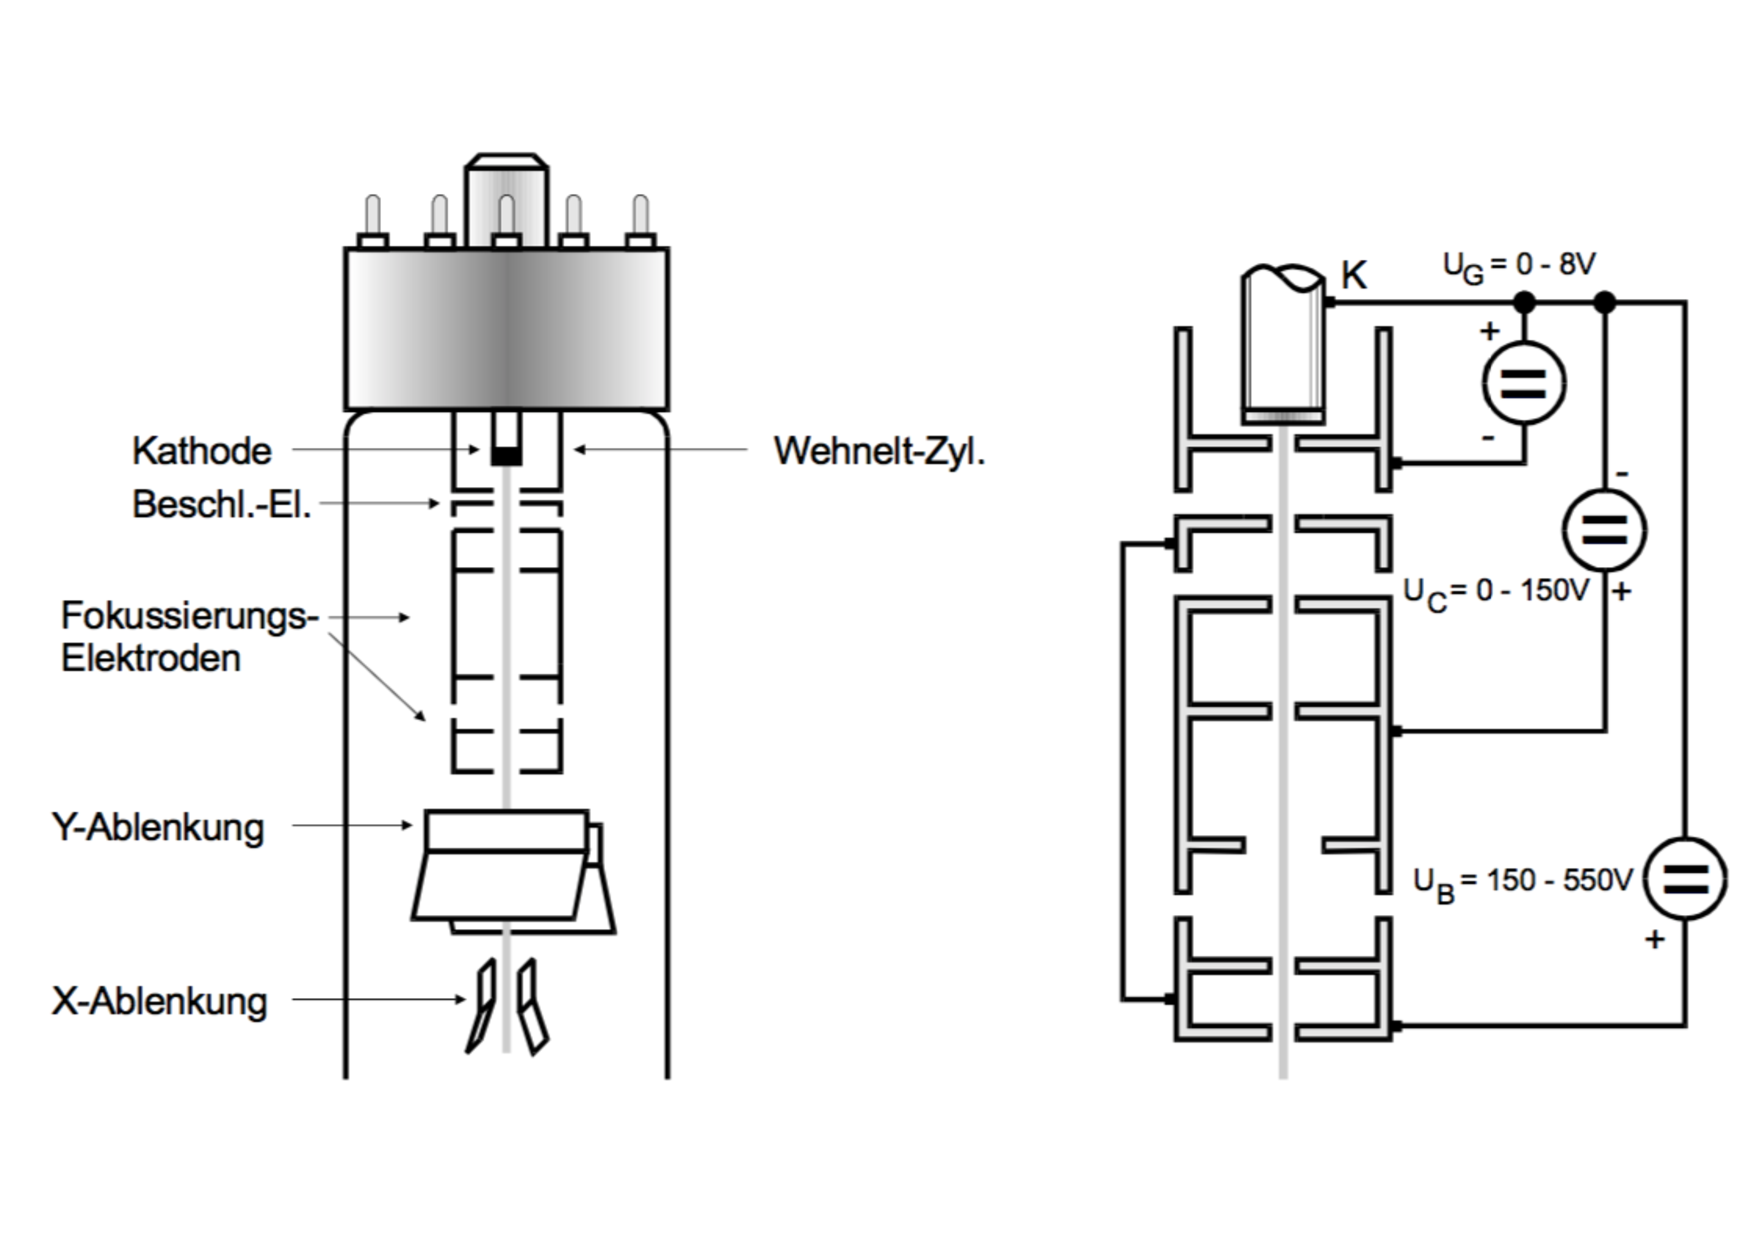
\includegraphics[width=0.8\textwidth]{EFeld1.pdf}
  \caption{Kathodenstrahlröhre \cite{1}}
  \label{fig:KSR}
\end{figure}
\\Die Kathodenstrahlröhre wird an die versorgende Spannungsquelle geschlossen (Abb. \ref{fig:emess1}).
Die Spannungsquelle zeigt die regelbare die Beschleunigungsspannung $U_{B}$ an.
Die Kathodenstrahlröhre wird mit den Spannungsgeneratoren der Ablenkspannungen verbunden.
Zusätzlich wird ein Voltmeter an den Spannungsgenerator für die Ablenkung in Y-Richtung gebracht.
Gemessen wird die Verschiebung des Elektronenstrahls auf dem Leuchtschirm und die Ablenkspannung $U_{d}$ für fünf unterschiedliche Beschleunigungsspannungen.
\begin{figure}
  \centering
  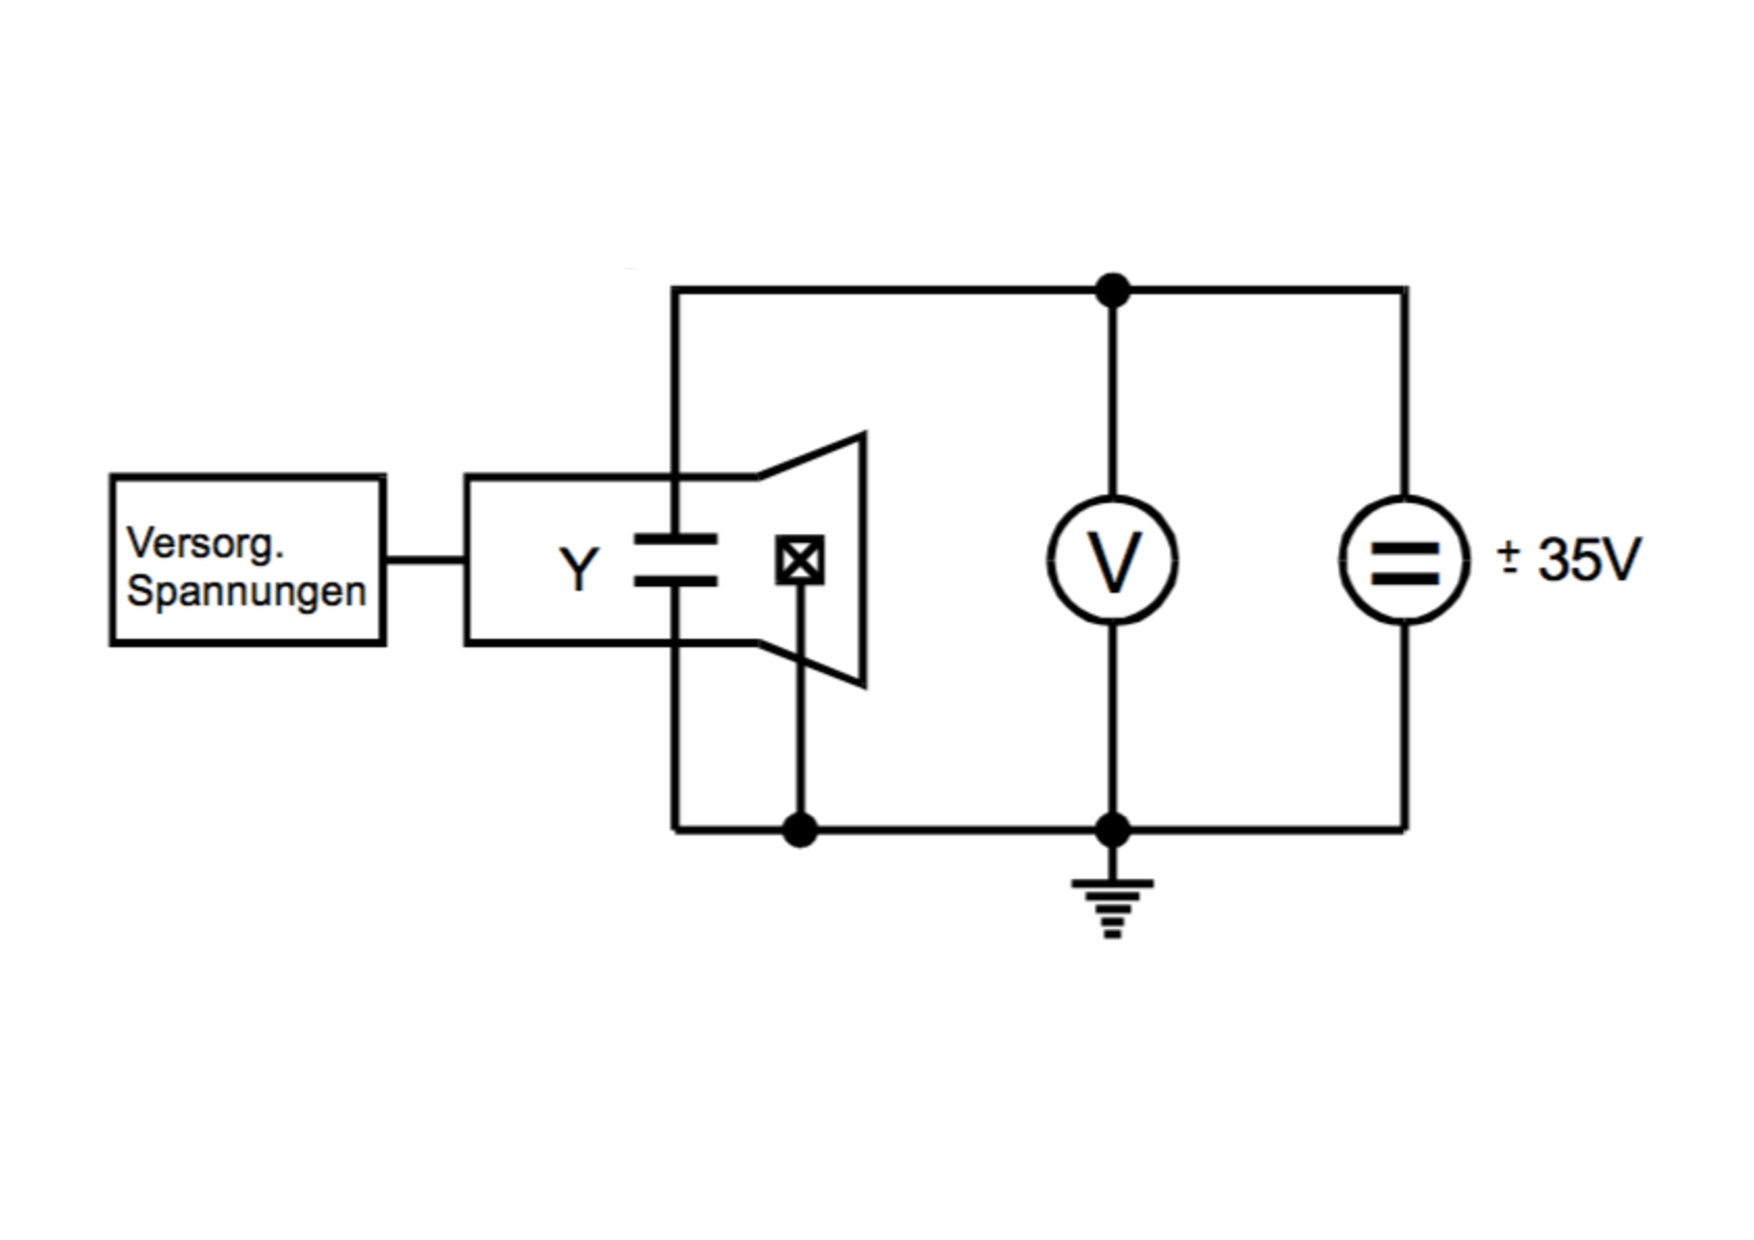
\includegraphics[width=0.8\textwidth]{EFeld3.pdf}
  \caption{Versuchsaufbau zur Messung der Ablenkung des Elektronenstrahls durch elektrische Felder \cite{1}}
  \label{fig:emess1}
\end{figure}

\subsubsection{Kathodenstrahl-Oszillograph und stehende Wellen}
Der Versuchsaufbau wird abgeändert, indem das Voltmeter ausgebaut wird und eine Sägezahnspannung $\nu_{Säg}$ an die X-Ablenkung gelegt wird (Abb. \ref{fig:emess2}).
Außerdem wird an die Y-Ablenkung eine Wechselspannung der Frequenz von $\nu_{Sin} \approx 80-90\si{Hz}$ laut Apparatur und der Spannungsamplitude $U_{max}=\SI{10}{V}$ gelegt.
Die angelegte Beschleunigungsspannung in der Kathodenstrahlröhre liegt bei $U_{B}={280}{V}$.
Die Frequenz $\nu_{Säg}$ wird so lange verändert, bis sich auf dem Oszilloskop eine stehende Welle abbildet.
Die stehenden Wellen werden fotografiert und es werden sieben zugehörigen Frequenzen der Sägezahnspannung und die maximale Strahlauslenkung notiert.
\begin{figure}
  \centering
  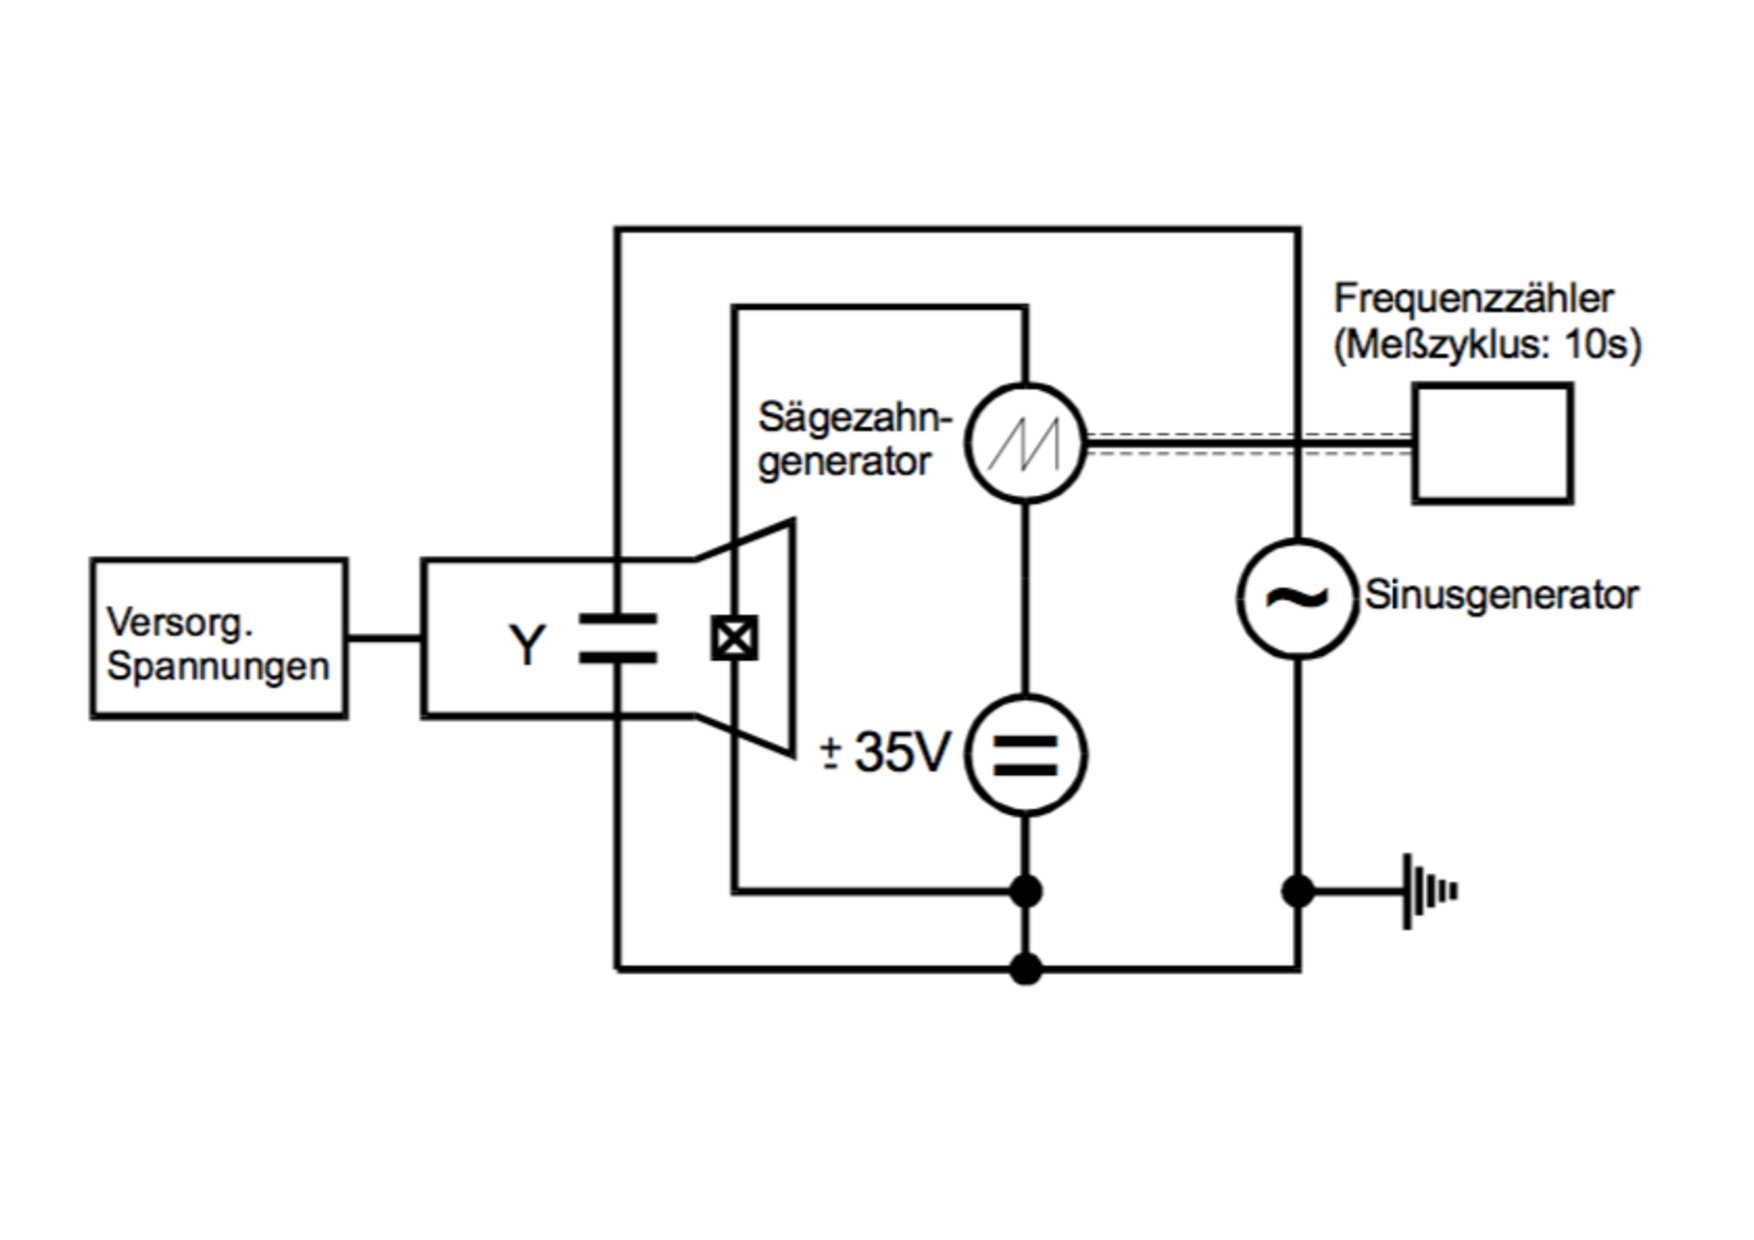
\includegraphics[width=0.8\textwidth]{EFeld4.pdf}
  \caption{Versuchsaufbau des Oszillographen und zum Erstellen der stehenden Wellen \cite{1}}
  \label{fig:emess2}
\end{figure}
\FloatBarrier

\subsection{Aufbau und Durchführung des Versuchs V502}
\subsubsection{Messung der spezifischen Ladung eines Elektrons}
Ein homogenes Magnetfeld wird durch ein Paar Helmholtzspulen mit dem Radius $r=\SI{0.282}{m}$ und der Windungszahl $N=20$ erzeugt.
Die Spulen werden mit einem regelbaren Strom $I$ gespeist.
In der Mitte der Helmholtzspulen befindet sich die Kathodenstrahlröhre (Abb. \ref{fig:KSR}).
Diese wird mit der Spannungsquelle verbunden, die die Beschleunigungsspannungen erzeugt.
Die Ablenkungsplatten werden an die entsprechenden Spannungsgeneratoren für die X- und Y-Ablenkung geschlossen.
Mithilfe des Kompasses wird ermittelt in welcher Richtung Norden liegt und das Spulenpaar wird parallel dazu ausgerichtet.
Der leuchtende Punkt auf dem Schirm wird mit der X- und Y- Ablenkung auf den untersten Punkt der Y-Achse des Koordinatensystems gebracht.
Die Stromquelle der Spulen wird eingeschaltet.
Der leuchtende Punkt wird durch das Erhöhen des Stroms $I$ um den Abstand $D$ auf dem Leuchtschirm verschoben.
Für fünf verschiedene Beschleunigungsspannungen werden zehn Messwerte des Abstands $D$ und des Stroms $I$ aufgenommen.

\subsubsection{Messung der Feldstärke des lokalen Erdmagnetfelds}
Mit dem Deklinatorium-Inklinatorium wird der Inklinationswinkel festgestellt.
Dazu wird zunächst die horizontale Richtung des Erdmagnetfelds gemessen und der Kompass wird gedreht, bis die Nadel bei 0° steht.
Dann wird der Kompass senkrecht gedreht.
Der Inklinationswinkel wird an der Skala abgelesen.
Die Ausrichtung der Helmholtzspulen wird zunächst beibehalten.
Die Beschleunigungsspannung wird auf $U_{B}=\SI{300}{V}$ verringert und der Strom $I$ wird ausgestellt.
Mit der X- und Y-Ablenkung wird der leuchtende Punkt auf dem Schirm in die Mitte des Koordinatensystems gebracht.
Die Apparatur wird nun um 90° gedreht.
Dabei verschiebt sich der leuchtende Punkt auf dem Schirm.
Der Strom $I$ in den Helmholtzspulen wird erhöht, bis der leuchtende Punkt wieder bei seinem Ausgangspunkt ist.
Der benötigte Strom $I$ wird notiert.
\FloatBarrier
